% Options for packages loaded elsewhere
\PassOptionsToPackage{unicode}{hyperref}
\PassOptionsToPackage{hyphens}{url}
%
\documentclass[
]{book}
\usepackage{lmodern}
\usepackage{amssymb,amsmath}
\usepackage{ifxetex,ifluatex}
\ifnum 0\ifxetex 1\fi\ifluatex 1\fi=0 % if pdftex
  \usepackage[T1]{fontenc}
  \usepackage[utf8]{inputenc}
  \usepackage{textcomp} % provide euro and other symbols
\else % if luatex or xetex
  \usepackage{unicode-math}
  \defaultfontfeatures{Scale=MatchLowercase}
  \defaultfontfeatures[\rmfamily]{Ligatures=TeX,Scale=1}
\fi
% Use upquote if available, for straight quotes in verbatim environments
\IfFileExists{upquote.sty}{\usepackage{upquote}}{}
\IfFileExists{microtype.sty}{% use microtype if available
  \usepackage[]{microtype}
  \UseMicrotypeSet[protrusion]{basicmath} % disable protrusion for tt fonts
}{}
\makeatletter
\@ifundefined{KOMAClassName}{% if non-KOMA class
  \IfFileExists{parskip.sty}{%
    \usepackage{parskip}
  }{% else
    \setlength{\parindent}{0pt}
    \setlength{\parskip}{6pt plus 2pt minus 1pt}}
}{% if KOMA class
  \KOMAoptions{parskip=half}}
\makeatother
\usepackage{xcolor}
\IfFileExists{xurl.sty}{\usepackage{xurl}}{} % add URL line breaks if available
\IfFileExists{bookmark.sty}{\usepackage{bookmark}}{\usepackage{hyperref}}
\hypersetup{
  pdftitle={Learning LogBook Tree phenology analysis with R},
  pdfauthor={Philipp Münker},
  hidelinks,
  pdfcreator={LaTeX via pandoc}}
\urlstyle{same} % disable monospaced font for URLs
\usepackage{color}
\usepackage{fancyvrb}
\newcommand{\VerbBar}{|}
\newcommand{\VERB}{\Verb[commandchars=\\\{\}]}
\DefineVerbatimEnvironment{Highlighting}{Verbatim}{commandchars=\\\{\}}
% Add ',fontsize=\small' for more characters per line
\usepackage{framed}
\definecolor{shadecolor}{RGB}{248,248,248}
\newenvironment{Shaded}{\begin{snugshade}}{\end{snugshade}}
\newcommand{\AlertTok}[1]{\textcolor[rgb]{0.94,0.16,0.16}{#1}}
\newcommand{\AnnotationTok}[1]{\textcolor[rgb]{0.56,0.35,0.01}{\textbf{\textit{#1}}}}
\newcommand{\AttributeTok}[1]{\textcolor[rgb]{0.77,0.63,0.00}{#1}}
\newcommand{\BaseNTok}[1]{\textcolor[rgb]{0.00,0.00,0.81}{#1}}
\newcommand{\BuiltInTok}[1]{#1}
\newcommand{\CharTok}[1]{\textcolor[rgb]{0.31,0.60,0.02}{#1}}
\newcommand{\CommentTok}[1]{\textcolor[rgb]{0.56,0.35,0.01}{\textit{#1}}}
\newcommand{\CommentVarTok}[1]{\textcolor[rgb]{0.56,0.35,0.01}{\textbf{\textit{#1}}}}
\newcommand{\ConstantTok}[1]{\textcolor[rgb]{0.00,0.00,0.00}{#1}}
\newcommand{\ControlFlowTok}[1]{\textcolor[rgb]{0.13,0.29,0.53}{\textbf{#1}}}
\newcommand{\DataTypeTok}[1]{\textcolor[rgb]{0.13,0.29,0.53}{#1}}
\newcommand{\DecValTok}[1]{\textcolor[rgb]{0.00,0.00,0.81}{#1}}
\newcommand{\DocumentationTok}[1]{\textcolor[rgb]{0.56,0.35,0.01}{\textbf{\textit{#1}}}}
\newcommand{\ErrorTok}[1]{\textcolor[rgb]{0.64,0.00,0.00}{\textbf{#1}}}
\newcommand{\ExtensionTok}[1]{#1}
\newcommand{\FloatTok}[1]{\textcolor[rgb]{0.00,0.00,0.81}{#1}}
\newcommand{\FunctionTok}[1]{\textcolor[rgb]{0.00,0.00,0.00}{#1}}
\newcommand{\ImportTok}[1]{#1}
\newcommand{\InformationTok}[1]{\textcolor[rgb]{0.56,0.35,0.01}{\textbf{\textit{#1}}}}
\newcommand{\KeywordTok}[1]{\textcolor[rgb]{0.13,0.29,0.53}{\textbf{#1}}}
\newcommand{\NormalTok}[1]{#1}
\newcommand{\OperatorTok}[1]{\textcolor[rgb]{0.81,0.36,0.00}{\textbf{#1}}}
\newcommand{\OtherTok}[1]{\textcolor[rgb]{0.56,0.35,0.01}{#1}}
\newcommand{\PreprocessorTok}[1]{\textcolor[rgb]{0.56,0.35,0.01}{\textit{#1}}}
\newcommand{\RegionMarkerTok}[1]{#1}
\newcommand{\SpecialCharTok}[1]{\textcolor[rgb]{0.00,0.00,0.00}{#1}}
\newcommand{\SpecialStringTok}[1]{\textcolor[rgb]{0.31,0.60,0.02}{#1}}
\newcommand{\StringTok}[1]{\textcolor[rgb]{0.31,0.60,0.02}{#1}}
\newcommand{\VariableTok}[1]{\textcolor[rgb]{0.00,0.00,0.00}{#1}}
\newcommand{\VerbatimStringTok}[1]{\textcolor[rgb]{0.31,0.60,0.02}{#1}}
\newcommand{\WarningTok}[1]{\textcolor[rgb]{0.56,0.35,0.01}{\textbf{\textit{#1}}}}
\usepackage{longtable,booktabs}
% Correct order of tables after \paragraph or \subparagraph
\usepackage{etoolbox}
\makeatletter
\patchcmd\longtable{\par}{\if@noskipsec\mbox{}\fi\par}{}{}
\makeatother
% Allow footnotes in longtable head/foot
\IfFileExists{footnotehyper.sty}{\usepackage{footnotehyper}}{\usepackage{footnote}}
\makesavenoteenv{longtable}
\usepackage{graphicx,grffile}
\makeatletter
\def\maxwidth{\ifdim\Gin@nat@width>\linewidth\linewidth\else\Gin@nat@width\fi}
\def\maxheight{\ifdim\Gin@nat@height>\textheight\textheight\else\Gin@nat@height\fi}
\makeatother
% Scale images if necessary, so that they will not overflow the page
% margins by default, and it is still possible to overwrite the defaults
% using explicit options in \includegraphics[width, height, ...]{}
\setkeys{Gin}{width=\maxwidth,height=\maxheight,keepaspectratio}
% Set default figure placement to htbp
\makeatletter
\def\fps@figure{htbp}
\makeatother
\setlength{\emergencystretch}{3em} % prevent overfull lines
\providecommand{\tightlist}{%
  \setlength{\itemsep}{0pt}\setlength{\parskip}{0pt}}
\setcounter{secnumdepth}{5}
\usepackage{booktabs}
\usepackage{booktabs}
\usepackage{longtable}
\usepackage{array}
\usepackage{multirow}
\usepackage{wrapfig}
\usepackage{float}
\usepackage{colortbl}
\usepackage{pdflscape}
\usepackage{tabu}
\usepackage{threeparttable}
\usepackage{threeparttablex}
\usepackage[normalem]{ulem}
\usepackage{makecell}
\usepackage{xcolor}
\usepackage[]{natbib}
\bibliographystyle{plainnat}

\title{Learning LogBook Tree phenology analysis with R}
\author{Philipp Münker}
\date{2022-12-28}

\begin{document}
\maketitle

{
\setcounter{tocdepth}{1}
\tableofcontents
}
\hypertarget{introduction}{%
\chapter{Introduction}\label{introduction}}

In this learning Logbook, all units from the Tree phenology analysis with R module are documented. In addition to the tasks set at the end of each learning unit, this work is supplemented with additional materials and analyses. This is done using weather data taken from my own weather station. The corresponding data can be found at the following link: \url{https://wettermuehle.de}. Access data can be requested if desired.

\hypertarget{tree-phenology}{%
\chapter{Tree phenology}\label{tree-phenology}}

If we consider fruit trees, their annual cycle can generally be described relatively easily. Starting in autumn, it is observed that almost all fruit trees shed their leaves and go into winter without foliage. Already in the autumn, the formation of the bud can often be observed. This bud then remains in a kind of winter dormancy throughout the winter and begins to grow with increasing temperatures in the spring. This process is usually followed by the flowering of the fruit trees with subsequent leaf development. Later in the year, fruits establish themselves from the buds, which mature at different times of the year.
But how does the tree know when it can begin flowering induction and no longer expect strong frost?
This can be described with the concept of dormancy. This can be divided into 4 phases.

\textbf{Tree dormancy}

\begin{itemize}
\tightlist
\item
  Dormancy establishment
\item
  Endodormancy
\item
  Ecodormancy
\item
  Growth resumption
\end{itemize}

\textbf{Dormacy establishment}

\begin{itemize}
\tightlist
\item
  Controlled by tempeature and photoperiod.
\end{itemize}

\textbf{Endodormancy}

\begin{itemize}
\tightlist
\item
  Controlled by plant endogenous factors. Plants unable to growth even under
  favorable environmental conditions.
\end{itemize}

\textbf{Ecodormancy}

\begin{itemize}
\tightlist
\item
  After a certain level of chill, endodormancy has been overcome and buds recover the capacity to grow. Trees become acclimated to freezing tolerance and are not deeply dormant, but growth is still prevented by unsuitable environmental conditions. Temperature is the most important driver in this process.
\end{itemize}

\hypertarget{treedormancy}{%
\chapter{Tree dormancy}\label{treedormancy}}

\hypertarget{task-1}{%
\section{Task 1}\label{task-1}}

\textbf{Put yourself in the place of a breeder who wants to calculate the temperature requirements of a newly released cultivar. Which method will you use to calculate the chilling and forcing periods? Please justify your answer.}

\begin{quote}
Long-term phenological data does not exist, so a statistical approach is not optimal for newly released cultivars. It is better to work with an empirical approach. To do this, collect flower buds and place shoots in a chamber for 10 days under favorable conditions (temperature between 20 and 25 degrees). After 10 days, measure the weight of the shoots in the chamber and the shoots without the chamber. If the weight difference is greater than 30\%, the cultivar is considered non-dormant. Otherwise, it is considered dormant
\end{quote}

\hypertarget{task-2}{%
\section{Task 2}\label{task-2}}

\textbf{Which are the advantages (2) of the BBCH scale compared with earlies scales?}

\begin{quote}
Not all parts of a tree are in the same development stage. Early scales only record the predominant state of the fruit tree. General principles for the design of a scale for plant growth stages include:

\begin{itemize}
\item
  Growth stages are easily recognizable under field conditions
\item
  Growth stages are graded in the order of appearance (early scales do not do this)
\item
  Two-digit code: Principal growth stages \textbar{} Secondary growth stages
\item
  Applicable for all cereals in all parts of the world. (Old scales can only be used for a specific group/fruit)
\end{itemize}
\end{quote}

\hypertarget{task-3}{%
\section{Task 3}\label{task-3}}

\textbf{Classify the following phenological stages of sweet cherry according to the BBCH scale:}

\begin{figure}
\centering
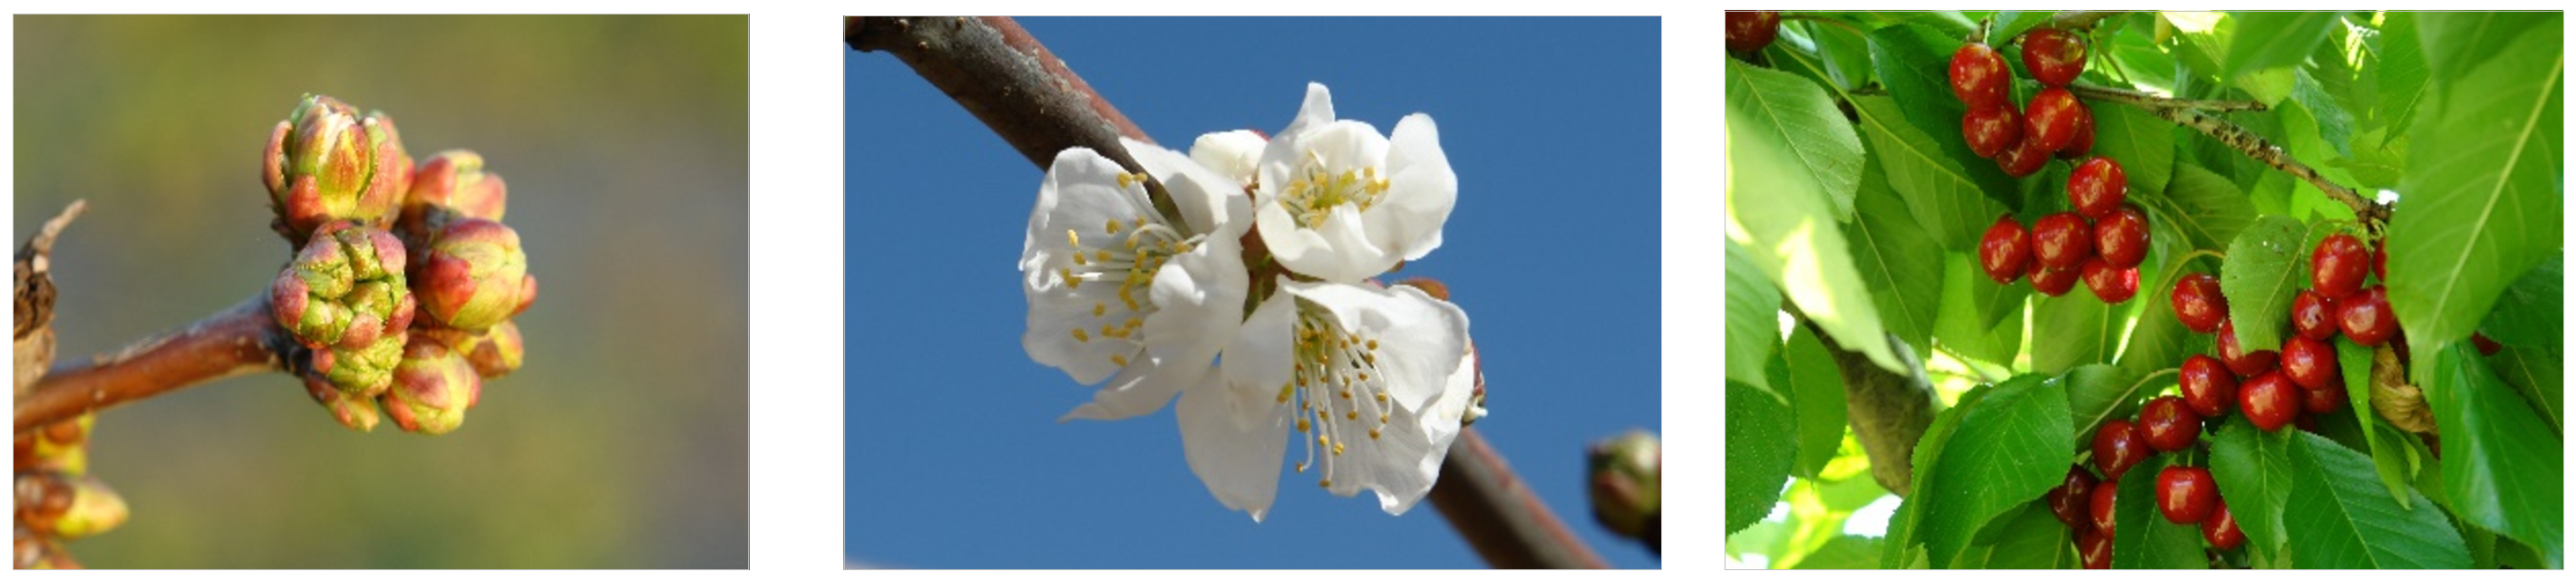
\includegraphics{./pheno_stages.png}
\caption{Picture 1 BBCH =55; Picture 2 BBCH =67; Picture 3 BBCH =89}
\end{figure}

\hypertarget{climate-change-and-impact-projection}{%
\chapter{Climate change and impact projection}\label{climate-change-and-impact-projection}}

\hypertarget{task-1-1}{%
\section{Task 1}\label{task-1-1}}

\textbf{List the main drivers of climate change at the decade to century scale, and briefly explain the mechanism through which the currently most important driver affects our climate}

\begin{table}

\caption{\label{tab:unnamed-chunk-2}Drivers of Climate Change}
\centering
\begin{tabular}[t]{l}
\hline
Drivers of climate change\\
\hline
Sun\\
\hline
Aerosols\\
\hline
Clouds\\
\hline
Ozone\\
\hline
Surface albedo\\
\hline
Greenhouse gases\\
\hline
\end{tabular}
\end{table}

\begin{quote}
The most important factor that currently has the greatest influence on climate and climate change is greenhouse gases. The most important greenhouse gases are water vapor, (carbon dioxide) CO2, (methane) CH4, and (nitrous oxides) N2O. Greenhouse gases can only absorb radiation of certain wavelengths. They absorb radiation with long wavelengths, which comes from the Earth's surface in the form of infrared radiation emitted by the warm Earth's surface. This radiation cannot leave the atmosphere and is trapped by the greenhouse gases, which returns it back to the Earth.
\end{quote}

\hypertarget{task-2-1}{%
\section{Task 2}\label{task-2-1}}

\textbf{Explain briefly what is special about temperature dynamics of the recent decades, and why we have good reasons to be concerned}

\begin{quote}
Over the past decades and throughout the last century, the temperature has been rising worldwide. Initially, this increase was relatively slow. The ten warmest years worldwide since 1880 were all measured after the millennium. The five warmest years worldwide were all recorded after 2014. This effect is also noticeable in Germany. Here, too, the ten warmest years were all measured after 2000, with one exception. If one places the temperature increase of the last decades in the climate history of the last one million years, it can be seen that there has never been such a strong temperature increase over such a relatively short period of time.

This rapid rise in temperature is developing its own dynamic. For example, high temperatures in the tundra cause the permafrost to thaw, releasing a large amount of CO2, a greenhouse gas that promotes even faster warming.
\end{quote}

\hypertarget{manual-chill-analysis}{%
\chapter{Manual Chill Analysis}\label{manual-chill-analysis}}

\begin{quote}
The \texttt{Winters\_hours\_gaps} data set has the columns: \texttt{Year}, \texttt{Month}, \texttt{Day}, \texttt{Hour}, \texttt{Temp\_gaps}, \texttt{Temp}. First, the function \texttt{cleaned\_data} is used to remove unnecessary columns such as \texttt{Temp\_gaps()} from the data set.
\end{quote}

\begin{Shaded}
\begin{Highlighting}[]
\CommentTok{#Clean Function}
\NormalTok{cleaned_data =}\StringTok{ }\ControlFlowTok{function}\NormalTok{(data_source) \{}
\NormalTok{  data_source =}\StringTok{ }
\StringTok{    }\NormalTok{data_source[, }\KeywordTok{c}\NormalTok{(}\StringTok{"Year"}\NormalTok{, }\StringTok{"Month"}\NormalTok{, }\StringTok{"Day"}\NormalTok{, }\StringTok{"Hour"}\NormalTok{, }\StringTok{"Temp"}\NormalTok{)]}
  \KeywordTok{return}\NormalTok{(data_source)}
\NormalTok{\}}

\CommentTok{# Apply Function to Winters_hours_gaps}
\KeywordTok{kable}\NormalTok{(}\KeywordTok{head}\NormalTok{(}\KeywordTok{cleaned_data}\NormalTok{(}\DataTypeTok{data_source =}\NormalTok{ Winters_hours_gaps)), }
      \StringTok{"pipe"}\NormalTok{, }\DataTypeTok{caption =} \StringTok{"Cleaned  Dataset: Winters_hours_gaps"}\NormalTok{)}
\end{Highlighting}
\end{Shaded}

\begin{longtable}[]{@{}rrrrr@{}}
\caption{\label{tab:unnamed-chunk-4}Cleaned Dataset: Winters\_hours\_gaps}\tabularnewline
\toprule
Year & Month & Day & Hour & Temp\tabularnewline
\midrule
\endfirsthead
\toprule
Year & Month & Day & Hour & Temp\tabularnewline
\midrule
\endhead
2008 & 3 & 3 & 10 & 15.127\tabularnewline
2008 & 3 & 3 & 11 & 17.153\tabularnewline
2008 & 3 & 3 & 12 & 18.699\tabularnewline
2008 & 3 & 3 & 13 & 18.699\tabularnewline
2008 & 3 & 3 & 14 & 18.842\tabularnewline
2008 & 3 & 3 & 15 & 19.508\tabularnewline
\bottomrule
\end{longtable}

\hypertarget{task-1-2}{%
\section{Task 1}\label{task-1-2}}

\textbf{Write a basic function that calculates warm hours (\textgreater25°C)}

\begin{Shaded}
\begin{Highlighting}[]
\NormalTok{WH =}\StringTok{ }\ControlFlowTok{function}\NormalTok{(hourtemps)}
\NormalTok{\{}
\NormalTok{  hourtemps[, }\StringTok{"warm_hours"}\NormalTok{] <-}\StringTok{ }\NormalTok{hourtemps}\OperatorTok{$}\NormalTok{Temp }\OperatorTok{>=}\StringTok{ }\FloatTok{25.0}
  \KeywordTok{return}\NormalTok{(hourtemps)}
\NormalTok{\}}
\end{Highlighting}
\end{Shaded}

\hypertarget{task-2-2}{%
\section{Task 2}\label{task-2-2}}

\textbf{Apply this function to the Winters\_hours\_gaps dataset}

\begin{Shaded}
\begin{Highlighting}[]
\CommentTok{# have a look to the data set}
\KeywordTok{kable}\NormalTok{(}\KeywordTok{head}\NormalTok{(Winters_hours_gaps), }
      \StringTok{"pipe"}\NormalTok{, }\DataTypeTok{caption =} 
        \StringTok{"Example Dataset: Winters_hours_gaps"}\NormalTok{) }
\end{Highlighting}
\end{Shaded}

\begin{longtable}[]{@{}rrrrrr@{}}
\caption{\label{tab:unnamed-chunk-6}Example Dataset: Winters\_hours\_gaps}\tabularnewline
\toprule
Year & Month & Day & Hour & Temp\_gaps & Temp\tabularnewline
\midrule
\endfirsthead
\toprule
Year & Month & Day & Hour & Temp\_gaps & Temp\tabularnewline
\midrule
\endhead
2008 & 3 & 3 & 10 & 15.127 & 15.127\tabularnewline
2008 & 3 & 3 & 11 & 17.153 & 17.153\tabularnewline
2008 & 3 & 3 & 12 & 18.699 & 18.699\tabularnewline
2008 & 3 & 3 & 13 & 18.699 & 18.699\tabularnewline
2008 & 3 & 3 & 14 & 18.842 & 18.842\tabularnewline
2008 & 3 & 3 & 15 & 19.508 & 19.508\tabularnewline
\bottomrule
\end{longtable}

\begin{Shaded}
\begin{Highlighting}[]
\CommentTok{# Apply Function}
\NormalTok{hourtemps =}\StringTok{ }\KeywordTok{cleaned_data}\NormalTok{(}\DataTypeTok{data_source =}\NormalTok{ Winters_hours_gaps)}
\KeywordTok{kable}\NormalTok{(}\KeywordTok{head}\NormalTok{(}\KeywordTok{WH}\NormalTok{(}\DataTypeTok{hourtemps =}\NormalTok{ hourtemps)), }\StringTok{"pipe"}\NormalTok{)}
\end{Highlighting}
\end{Shaded}

\begin{longtable}[]{@{}rrrrrl@{}}
\toprule
Year & Month & Day & Hour & Temp & warm\_hours\tabularnewline
\midrule
\endhead
2008 & 3 & 3 & 10 & 15.127 & FALSE\tabularnewline
2008 & 3 & 3 & 11 & 17.153 & FALSE\tabularnewline
2008 & 3 & 3 & 12 & 18.699 & FALSE\tabularnewline
2008 & 3 & 3 & 13 & 18.699 & FALSE\tabularnewline
2008 & 3 & 3 & 14 & 18.842 & FALSE\tabularnewline
2008 & 3 & 3 & 15 & 19.508 & FALSE\tabularnewline
\bottomrule
\end{longtable}

\hypertarget{task-3-1}{%
\section{Task 3}\label{task-3-1}}

\textbf{Extend this function, so that it can take start and end dates as inputs and sums up warm hours between these dates}

\begin{Shaded}
\begin{Highlighting}[]
\NormalTok{warm_hours_function =}\StringTok{ }\ControlFlowTok{function}\NormalTok{(Input_Data,}
\NormalTok{                               S_Jahr,}
\NormalTok{                               S_Monat,}
\NormalTok{                               S_Tag,}
\NormalTok{                               S_Stunde,}
\NormalTok{                               E_Jahr,}
\NormalTok{                               E_Monat,}
\NormalTok{                               E_Tag,}
\NormalTok{                               E_Stunde) \{}
\NormalTok{  Start_Date <-}
\StringTok{    }\KeywordTok{which}\NormalTok{(}
\NormalTok{      hourtemps}\OperatorTok{$}\NormalTok{Year }\OperatorTok{==}\StringTok{ }\NormalTok{S_Jahr }\OperatorTok{&}\StringTok{ }\NormalTok{hourtemps}\OperatorTok{$}\NormalTok{Month }\OperatorTok{==}\StringTok{ }\NormalTok{S_Monat }\OperatorTok{&}
\StringTok{        }\NormalTok{hourtemps}\OperatorTok{$}\NormalTok{Day }\OperatorTok{==}\StringTok{ }\NormalTok{S_Tag }\OperatorTok{&}
\StringTok{        }\NormalTok{hourtemps}\OperatorTok{$}\NormalTok{Hour }\OperatorTok{==}\StringTok{ }\NormalTok{S_Stunde}
\NormalTok{    )}
\NormalTok{  End_Date <-}\StringTok{ }\KeywordTok{which}\NormalTok{(}
\NormalTok{    hourtemps}\OperatorTok{$}\NormalTok{Year }\OperatorTok{==}\StringTok{ }\NormalTok{E_Jahr }\OperatorTok{&}\StringTok{ }\NormalTok{hourtemps}\OperatorTok{$}\NormalTok{Month }\OperatorTok{==}\StringTok{ }\NormalTok{E_Monat }\OperatorTok{&}
\StringTok{      }\NormalTok{hourtemps}\OperatorTok{$}\NormalTok{Day }\OperatorTok{==}\StringTok{ }\NormalTok{E_Tag }\OperatorTok{&}\StringTok{ }\NormalTok{hourtemps}\OperatorTok{$}\NormalTok{Hour }\OperatorTok{==}\StringTok{ }\NormalTok{E_Stunde}
\NormalTok{  )}
  
  \CommentTok{# Apply Function Warm Hours (WH)}
\NormalTok{  hourtemps =}\StringTok{ }\KeywordTok{WH}\NormalTok{(}\DataTypeTok{hourtemps =}\NormalTok{ Input_Data)}
  
  \CommentTok{# Calculate warm_hours}
\NormalTok{  warm_hours =}\StringTok{ }\KeywordTok{sum}\NormalTok{(hourtemps}\OperatorTok{$}\NormalTok{warm_hours[Start_Date}\OperatorTok{:}\NormalTok{End_Date])}
  
  \KeywordTok{return}\NormalTok{(}\KeywordTok{cat}\NormalTok{(}\StringTok{"The number of heat hours is:"}\NormalTok{, }\KeywordTok{paste}\NormalTok{(warm_hours)))}
\NormalTok{\}}

\KeywordTok{warm_hours_function}\NormalTok{(}
  \DataTypeTok{Input_Data =}\NormalTok{ hourtemps,}
  \DataTypeTok{S_Jahr =} \DecValTok{2008}\NormalTok{,}
  \DataTypeTok{S_Monat =} \DecValTok{5}\NormalTok{,}
  \DataTypeTok{S_Tag =} \DecValTok{1}\NormalTok{,}
  \DataTypeTok{S_Stunde =} \DecValTok{12}\NormalTok{,}
  \DataTypeTok{E_Jahr =} \DecValTok{2008}\NormalTok{,}
  \DataTypeTok{E_Monat =} \DecValTok{8}\NormalTok{,}
  \DataTypeTok{E_Tag =} \DecValTok{31}\NormalTok{,}
  \DataTypeTok{E_Stunde =} \DecValTok{12}
\NormalTok{)}
\end{Highlighting}
\end{Shaded}

\begin{verbatim}
## The number of heat hours is: 957
\end{verbatim}

\hypertarget{chill-models}{%
\chapter{Chill Models}\label{chill-models}}

\begin{quote}
Counting chill hours can be done in various ways. \texttt{ChillR} offers some functions for this purpose. The simplest function for this is the \texttt{Chilling\_Hours()} function. It records one chill hour for every temperature between 0 and 7.2 degrees.
A slightly more complex function is the \texttt{Utah\_Model()} function. It evaluates the measured temperatures and decides whether a full chill hour was reached or only half. For example, if the temperature is between 1 and 2 degrees, one chill hour has been reached. If it is between 3 and 4 degrees, two chill hours are recorded.
The \texttt{Dynamic\_model()} function is the most complex function. It is taken from an Excel sheet.
The \texttt{chilling()} function combines the functions described above and presents the results in an overview.
\end{quote}

\hypertarget{task-1-3}{%
\section{Task 1}\label{task-1-3}}

\textbf{Run the chilling() function on the Winters\_hours\_gap dataset}

\begin{Shaded}
\begin{Highlighting}[]
\CommentTok{# run chilling function on Winters_hours_gap dataset}
\NormalTok{output =}
\StringTok{  }\KeywordTok{chilling}\NormalTok{(}\KeywordTok{make_JDay}\NormalTok{(Winters_hours_gaps),}
           \DataTypeTok{Start_JDay =} \DecValTok{90}\NormalTok{,}
           \DataTypeTok{End_JDay =} \DecValTok{100}\NormalTok{)}

\KeywordTok{kable}\NormalTok{(output, }\DataTypeTok{caption =}\StringTok{"chilling function on Winters_hours_gap"}\NormalTok{) }\OperatorTok
\KeywordTok{kable_classic_2}\NormalTok{(}\DataTypeTok{full_width =}\NormalTok{ F, }\DataTypeTok{font_size =} \DecValTok{7}\NormalTok{)}
\end{Highlighting}
\end{Shaded}

\textbackslash begin\{table\}

\textbackslash caption\{\label{tab:unnamed-chunk-9}chilling function on Winters\_hours\_gap\}
\centering
\fontsize{7}{9}\selectfont

\begin{tabular}[t]{l|r|r|r|r|r|r|r|r}
\hline
Season & End\_year & Season\_days & Data\_days & Perc\_complete & Chilling\_Hours & Utah\_Model & Chill\_portions & GDH\\
\hline
2007/2008 & 2008 & 11 & 11 & 100 & 40 & 15.5 & 2.009147 & 2406.52\\
\hline
\end{tabular}

\textbackslash end\{table\}

\hypertarget{task2}{%
\section{Task2}\label{task2}}

\textbf{Create your own temperature-weighting chill model using the \texttt{step\_model()} function}

\begin{quote}
The \texttt{step\_model} function has two arguments that the user can pass. One is a dataset of temperature data \texttt{HourTemp} and the other is a \texttt{data.frame()} (df) consisting of \texttt{lower}, \texttt{upper}, and \texttt{weight}. A pre-defined lower temperature range from, for example, -1000 °C to 0 °C is set, with all temperatures within this range being assigned a weight of 0. Assuming that hourly temperature data is provided as input, the
temperature can be multiplied by the corresponding weight to obtain the amount of ``chillhours''. For example: -1 °C is within the range {[}-1000, 0{]} == 0, resulting in 0 chillhours. Another argument is \texttt{summ}. If \texttt{summ\ =\ TRUE}, the cumulative chillhours over a defined period will be output. If \texttt{summ\ =\ FALSE}, the weights of the chillhours will be output.
\end{quote}

\begin{Shaded}
\begin{Highlighting}[]
\NormalTok{step_model =}\StringTok{ }\ControlFlowTok{function}\NormalTok{ (HourTemp,}
                        \DataTypeTok{df =}
                          \KeywordTok{data.frame}\NormalTok{(}
                            \DataTypeTok{lower =} \KeywordTok{c}\NormalTok{(}\OperatorTok{-}\DecValTok{1000}\NormalTok{, }\FloatTok{1.4}\NormalTok{, }\FloatTok{2.4}\NormalTok{, }\FloatTok{9.1}\NormalTok{, }\FloatTok{12.4}\NormalTok{, }\FloatTok{15.9}\NormalTok{, }\DecValTok{18}\NormalTok{),}
                            \DataTypeTok{upper =} \KeywordTok{c}\NormalTok{(}\FloatTok{1.4}\NormalTok{, }\FloatTok{2.4}\NormalTok{, }\FloatTok{9.1}\NormalTok{, }\FloatTok{12.4}\NormalTok{, }\FloatTok{15.9}\NormalTok{, }\DecValTok{18}\NormalTok{, }\DecValTok{1000}\NormalTok{),}
                            \DataTypeTok{weight =} \KeywordTok{c}\NormalTok{(}\DecValTok{0}\NormalTok{, }\FloatTok{0.5}\NormalTok{, }\DecValTok{1}\NormalTok{, }\FloatTok{0.5}\NormalTok{, }\DecValTok{0}\NormalTok{, }\FloatTok{-0.5}\NormalTok{, }\DecValTok{-1}\NormalTok{)}
\NormalTok{                          ),}
                        \DataTypeTok{summ =} \OtherTok{TRUE}\NormalTok{)}
\NormalTok{\{}
\NormalTok{  lower <-}\StringTok{ }\NormalTok{df}\OperatorTok{$}\NormalTok{lower}
\NormalTok{  upper <-}\StringTok{ }\NormalTok{df}\OperatorTok{$}\NormalTok{upper}
\NormalTok{  weight <-}\StringTok{ }\NormalTok{df}\OperatorTok{$}\NormalTok{weight}
  \ControlFlowTok{if}\NormalTok{ (summ }\OperatorTok{==}\StringTok{ }\OtherTok{TRUE}\NormalTok{)}
    \KeywordTok{return}\NormalTok{(}\KeywordTok{cumsum}\NormalTok{(}\KeywordTok{sapply}\NormalTok{(HourTemp, }\ControlFlowTok{function}\NormalTok{(x)}
\NormalTok{      weight[}\KeywordTok{which}\NormalTok{(x }\OperatorTok{>}
\StringTok{                     }\NormalTok{lower }\OperatorTok{&}\StringTok{ }\NormalTok{x }\OperatorTok{<=}\StringTok{ }\NormalTok{upper)])))}
  \ControlFlowTok{else}
    \KeywordTok{return}\NormalTok{(}\KeywordTok{sapply}\NormalTok{(HourTemp, }\ControlFlowTok{function}\NormalTok{(x)}
\NormalTok{      weight[}\KeywordTok{which}\NormalTok{(x }\OperatorTok{>}
\StringTok{                     }\NormalTok{lower }\OperatorTok{&}\StringTok{ }\NormalTok{x }\OperatorTok{<=}\StringTok{ }\NormalTok{upper)]))}
\NormalTok{\}}
\end{Highlighting}
\end{Shaded}

\begin{quote}
Here, only an ``own data field'' is defined with its own limits that have their own weight. For example, from -100 °C to 0 °C, the weight is set to 0. In this case, no ``chillhour'' occurs. If the temperature is between 0 °C and 2 °C, the weight of the ``chillhour'' is 0.5. In this case, half a ``chillhour'' occurs.
\end{quote}

\begin{Shaded}
\begin{Highlighting}[]
\NormalTok{own_df =}\StringTok{ }\KeywordTok{data.frame}\NormalTok{ (}\DataTypeTok{lower  =} \KeywordTok{c}\NormalTok{(}\OperatorTok{-}\DecValTok{100}\NormalTok{,}\DecValTok{0}\NormalTok{,  }\DecValTok{2}\NormalTok{, }\DecValTok{4}\NormalTok{,  }\DecValTok{5}\NormalTok{, }\DecValTok{6}\NormalTok{,   }\DecValTok{7}\NormalTok{    ),}
                     \DataTypeTok{upper  =} \KeywordTok{c}\NormalTok{(  }\DecValTok{0}\NormalTok{, }\DecValTok{2}\NormalTok{,  }\DecValTok{4}\NormalTok{, }\DecValTok{5}\NormalTok{,  }\DecValTok{6}\NormalTok{, }\DecValTok{7}\NormalTok{,   }\DecValTok{100}\NormalTok{  ),}
                     \DataTypeTok{weight =} \KeywordTok{c}\NormalTok{(  }\DecValTok{0}\NormalTok{, }\FloatTok{0.5}\NormalTok{,}\DecValTok{1}\NormalTok{, }\FloatTok{1.5}\NormalTok{,}\DecValTok{1}\NormalTok{, }\FloatTok{0.5}\NormalTok{, }\DecValTok{0}\NormalTok{    ))}
\end{Highlighting}
\end{Shaded}

\begin{quote}
After the dataframe with your own weights has been created, it can be implemented into the \texttt{step\_model()} function.
\end{quote}

\begin{Shaded}
\begin{Highlighting}[]
\NormalTok{use_step_model =}\StringTok{ }\ControlFlowTok{function}\NormalTok{(x)\{}\KeywordTok{step_model}\NormalTok{(x,own_df)\}}
  
\CommentTok{# quick aplly }
\KeywordTok{use_step_model}\NormalTok{(}\DataTypeTok{x =}\NormalTok{ Winters_hours_gaps}\OperatorTok{$}\NormalTok{Temp)[}\DecValTok{1}\OperatorTok{:}\DecValTok{100}\NormalTok{]}
\end{Highlighting}
\end{Shaded}

\begin{verbatim}
##   [1]  0.0  0.0  0.0  0.0  0.0  0.0  0.0  0.0  0.0  0.0  0.0  0.0  0.0  0.0  0.5
##  [16]  1.0  1.0  1.0  1.5  2.5  3.5  4.5  4.5  4.5  4.5  4.5  4.5  4.5  4.5  4.5
##  [31]  4.5  4.5  4.5  4.5  4.5  4.5  4.5  4.5  4.5  4.5  4.5  4.5  4.5  4.5  4.5
##  [46]  4.5  4.5  4.5  4.5  4.5  4.5  4.5  4.5  4.5  4.5  4.5  4.5  4.5  4.5  4.5
##  [61]  4.5  5.0  5.5  6.0  7.0  8.5  9.5 10.5 11.5 12.5 13.0 13.0 13.0 13.0 13.0
##  [76] 13.0 13.0 13.0 13.0 13.0 13.0 13.0 13.0 13.0 13.0 13.5 14.0 15.0 16.5 18.0
##  [91] 19.5 21.0 22.0 23.0 23.0 23.0 23.0 23.0 23.0 23.0
\end{verbatim}

\hypertarget{task3}{%
\section{Task3}\label{task3}}

\textbf{Run this model on the Winters\_hours\_gaps dataset using the tempResponse() function}

\begin{quote}
The \texttt{tempResponse()} function can display and summarize some chill models. Here is the model \texttt{weather\_mill()} our own chilling model which is created by the \texttt{step\_model()}. The modified \texttt{step\_model()} function is renamed to \texttt{use\_step\_model()} and passed as a parameter to the tempResponse function (weather\_mill = use\_step\_model).
\end{quote}

\begin{Shaded}
\begin{Highlighting}[]
\NormalTok{output <-}
\StringTok{  }\KeywordTok{tempResponse}\NormalTok{(}
    \KeywordTok{make_JDay}\NormalTok{(Winters_hours_gaps),}
    \DataTypeTok{Start_JDay =} \DecValTok{30}\NormalTok{,}
    \DataTypeTok{End_JDay =} \DecValTok{100}\NormalTok{,}
    \DataTypeTok{models =} \KeywordTok{list}\NormalTok{(}
      \DataTypeTok{Chill_Portions =}\NormalTok{ Dynamic_Model,}
      \DataTypeTok{GDH =}\NormalTok{ GDH,}
      \DataTypeTok{weather_mill =}\NormalTok{ use_step_model, }\CommentTok{# own model weather_mill}
      \DataTypeTok{Utah_Model =}\NormalTok{ Utah_Model}
\NormalTok{    )}
\NormalTok{  )}

\CommentTok{# display result}
\KeywordTok{kable}\NormalTok{(output, }\DataTypeTok{caption =} \StringTok{"Summarized some models"}\NormalTok{) }\OperatorTok
\StringTok{  }\KeywordTok{kable_styling}\NormalTok{(}\StringTok{"striped"}\NormalTok{, }\DataTypeTok{position =} \StringTok{"left"}\NormalTok{, }\DataTypeTok{font_size =} \DecValTok{7}\NormalTok{)}
\end{Highlighting}
\end{Shaded}

\begin{table}

\caption{\label{tab:unnamed-chunk-13}Summarized some models}
\fontsize{7}{9}\selectfont
\begin{tabular}[t]{l|r|r|r|r|r|r|r|r}
\hline
Season & End\_year & Season\_days & Data\_days & Perc\_complete & Chill\_Portions & GDH & weather\_mill & Utah\_Model\\
\hline
2007/2008 & 2008 & 71 & 37.58333 & 52.93427 & 5.930439 & 8392.585 & 84 & 49.5\\
\hline
\end{tabular}
\end{table}

\begin{quote}
If the Utah Model is included, which is based on the default settings of the Step Model, a clear difference between the modified Step Model and the Utah Model can be observed.
\end{quote}

\hypertarget{making-hourly-temperatures}{%
\chapter{Making hourly temperatures}\label{making-hourly-temperatures}}

\hypertarget{task-1-4}{%
\section{Task 1}\label{task-1-4}}

\textbf{Choose a location of interest, find out its latitude and produce plots of daily sunrise, sunset and daylength}

\begin{quote}
First, I would like to compare the lengths of days among locations of interest. I have selected Glogau in Poland, Zülpich in Germany, Tenerife in Spain, Moscow in Russia, and Karkaralinsk in Kazakhstan.
\end{quote}

\begin{Shaded}
\begin{Highlighting}[]
\CommentTok{# initialize the variables with daylength, sunrise and sunset by the function daylength}
\NormalTok{Glogau      <-}\StringTok{ }\KeywordTok{daylength}\NormalTok{(}\DataTypeTok{latitude =} \FloatTok{51.40}\NormalTok{, }\DataTypeTok{JDay =} \DecValTok{1}\OperatorTok{:}\DecValTok{365}\NormalTok{)}
\NormalTok{Teneriffa   <-}\StringTok{ }\KeywordTok{daylength}\NormalTok{(}\DataTypeTok{latitude =} \FloatTok{28.19}\NormalTok{, }\DataTypeTok{JDay =} \DecValTok{1}\OperatorTok{:}\DecValTok{365}\NormalTok{)}
\NormalTok{Zuelpich    <-}\StringTok{ }\KeywordTok{daylength}\NormalTok{(}\DataTypeTok{latitude =} \FloatTok{50.42}\NormalTok{, }\DataTypeTok{JDay =} \DecValTok{1}\OperatorTok{:}\DecValTok{365}\NormalTok{)}
\NormalTok{Moskau      <-}\StringTok{ }\KeywordTok{daylength}\NormalTok{(}\DataTypeTok{latitude =} \FloatTok{55.45}\NormalTok{, }\DataTypeTok{JDay =} \DecValTok{1}\OperatorTok{:}\DecValTok{365}\NormalTok{)}
\NormalTok{Karkaralinsk <-}\StringTok{ }\KeywordTok{daylength}\NormalTok{(}\DataTypeTok{latitude =} \FloatTok{49.24}\NormalTok{, }\DataTypeTok{JDay =} \DecValTok{1}\OperatorTok{:}\DecValTok{365}\NormalTok{)}

\CommentTok{# Create a dataframe consisting of the variables "base" (days 1 to 365) and the}
\CommentTok{# respective locations and containing only the day length for each location.}
\NormalTok{df <-}\StringTok{ }\KeywordTok{data.frame}\NormalTok{(}
  \DataTypeTok{base         =} \KeywordTok{seq}\NormalTok{(}\KeywordTok{length}\NormalTok{(Glogau[[}\DecValTok{1}\NormalTok{]])),}
  \DataTypeTok{Glogau       =}\NormalTok{ Glogau[[}\DecValTok{3}\NormalTok{]],}
  \DataTypeTok{Teneriffa    =}\NormalTok{ Teneriffa[[}\DecValTok{3}\NormalTok{]],}
\NormalTok{  Zülpich      =}\StringTok{ }\NormalTok{Zuelpich[[}\DecValTok{3}\NormalTok{]],}
  \DataTypeTok{Moskau       =}\NormalTok{ Moskau[[}\DecValTok{3}\NormalTok{]],}
  \DataTypeTok{Karkaralinsk =}\NormalTok{ Karkaralinsk[[}\DecValTok{3}\NormalTok{]]}
\NormalTok{)}


\KeywordTok{kable}\NormalTok{(}\KeywordTok{head}\NormalTok{(df), }\DataTypeTok{caption =} \StringTok{"Differnt Locations"}\NormalTok{) }\OperatorTok\StringTok{ }\KeywordTok{kable_styling}\NormalTok{(}\StringTok{"striped"}\NormalTok{, }\DataTypeTok{position =} \StringTok{"left"}\NormalTok{, }\DataTypeTok{font_size =} \DecValTok{7}\NormalTok{)}
\end{Highlighting}
\end{Shaded}

\begin{table}

\caption{\label{tab:unnamed-chunk-14}Differnt Locations}
\fontsize{7}{9}\selectfont
\begin{tabular}[t]{r|r|r|r|r|r}
\hline
base & Glogau & Teneriffa & Zülpich & Moskau & Karkaralinsk\\
\hline
1 & 7.930050 & 10.38197 & 8.086864 & 7.175796 & 8.265160\\
\hline
2 & 7.948054 & 10.38872 & 8.104044 & 7.198073 & 8.281428\\
\hline
3 & 7.967737 & 10.39612 & 8.122830 & 7.222407 & 8.299217\\
\hline
4 & 7.989077 & 10.40415 & 8.143199 & 7.248768 & 8.318509\\
\hline
5 & 8.012048 & 10.41281 & 8.165129 & 7.277120 & 8.339282\\
\hline
6 & 8.036625 & 10.42209 & 8.188595 & 7.307424 & 8.361515\\
\hline
\end{tabular}
\end{table}

\begin{Shaded}
\begin{Highlighting}[]
\CommentTok{# create a pivot table}
\NormalTok{df_long <-}
\StringTok{  }\KeywordTok{pivot_longer}\NormalTok{(df, }\OperatorTok{-}\StringTok{"base"}\NormalTok{, }\DataTypeTok{names_to =} \StringTok{"Location"}\NormalTok{, }\DataTypeTok{values_to =} \StringTok{"daylength"}\NormalTok{)}

\KeywordTok{kable}\NormalTok{(}\KeywordTok{head}\NormalTok{(df_long)) }\OperatorTok\StringTok{ }\KeywordTok{kable_styling}\NormalTok{(}\StringTok{"striped"}\NormalTok{, }\DataTypeTok{position =} \StringTok{"left"}\NormalTok{, }\DataTypeTok{font_size =} \DecValTok{10}\NormalTok{)}
\end{Highlighting}
\end{Shaded}

\begingroup\fontsize{10}{12}\selectfont

\begin{tabular}{r|l|r}
\hline
base & Location & daylength\\
\hline
1 & Glogau & 7.930050\\
\hline
1 & Teneriffa & 10.381965\\
\hline
1 & Zülpich & 8.086864\\
\hline
1 & Moskau & 7.175796\\
\hline
1 & Karkaralinsk & 8.265160\\
\hline
2 & Glogau & 7.948054\\
\hline
\end{tabular}
\endgroup{}

\begin{Shaded}
\begin{Highlighting}[]
\CommentTok{# plot the result with ggplot}
\KeywordTok{ggplot}\NormalTok{(df_long, }\KeywordTok{aes}\NormalTok{(}\DataTypeTok{x =}\NormalTok{ base, }\DataTypeTok{y =}\NormalTok{ daylength, }\DataTypeTok{groupe =}\NormalTok{ Location)) }\OperatorTok{+}
\StringTok{  }\KeywordTok{geom_line}\NormalTok{(}\KeywordTok{aes}\NormalTok{(}\DataTypeTok{color =}\NormalTok{ Location), }\DataTypeTok{lwd =} \FloatTok{1.0}\NormalTok{) }\OperatorTok{+}
\StringTok{  }\KeywordTok{ggtitle}\NormalTok{(}\StringTok{"Different day lengths in different places"}\NormalTok{) }\OperatorTok{+}
\StringTok{  }\KeywordTok{labs}\NormalTok{(}\DataTypeTok{x =} \StringTok{"Days"}\NormalTok{, }\DataTypeTok{y =} \StringTok{"Daylength [h]"}\NormalTok{) }\OperatorTok{+}\StringTok{ }\KeywordTok{theme_gray}\NormalTok{(}\DataTypeTok{base_size =} \DecValTok{15}\NormalTok{)}
\end{Highlighting}
\end{Shaded}

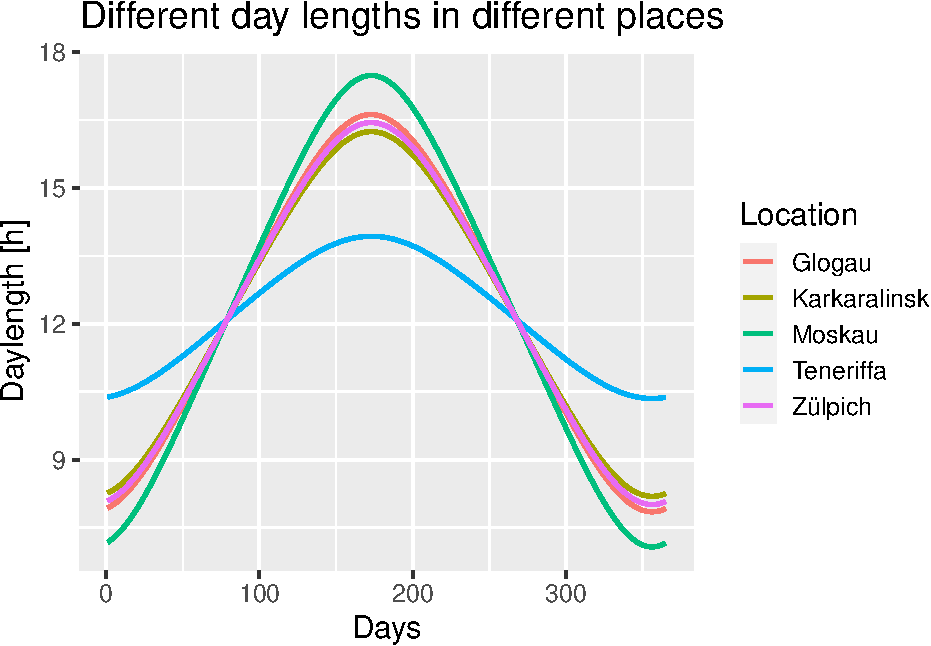
\includegraphics{Tree-Phenology_files/figure-latex/unnamed-chunk-14-1.pdf}

\begin{quote}
Create a summary of the sunrise, sunset, and day length for Moscow.
\end{quote}

\begin{Shaded}
\begin{Highlighting}[]
\NormalTok{Days <-}\StringTok{ }\KeywordTok{daylength}\NormalTok{(}\DataTypeTok{latitude =} \FloatTok{55.45}\NormalTok{, }\DataTypeTok{JDay =} \DecValTok{1}\OperatorTok{:}\DecValTok{365}\NormalTok{)}

\NormalTok{Days_df <-}
\StringTok{  }\KeywordTok{data.frame}\NormalTok{(}
    \DataTypeTok{JDay =} \DecValTok{1}\OperatorTok{:}\DecValTok{365}\NormalTok{,}
    \DataTypeTok{Sunrise =}\NormalTok{ Days}\OperatorTok{$}\NormalTok{Sunrise,}
    \DataTypeTok{Sunset =}\NormalTok{ Days}\OperatorTok{$}\NormalTok{Sunset,}
    \DataTypeTok{Daylength =}\NormalTok{ Days}\OperatorTok{$}\NormalTok{Daylength}
\NormalTok{  )}

\NormalTok{Days_df<-}\KeywordTok{melt}\NormalTok{(Days_df, }\DataTypeTok{id=}\KeywordTok{c}\NormalTok{(}\StringTok{"JDay"}\NormalTok{)) }
\end{Highlighting}
\end{Shaded}

\begin{quote}
Show the final result
\end{quote}

\begin{Shaded}
\begin{Highlighting}[]
\KeywordTok{ggplot}\NormalTok{(Days_df, }\KeywordTok{aes}\NormalTok{(}\DataTypeTok{x =}\NormalTok{ JDay, }\DataTypeTok{y =}\NormalTok{ value)) }\OperatorTok{+}\StringTok{ }\KeywordTok{geom_line}\NormalTok{(}\DataTypeTok{lwd =} \FloatTok{1.5}\NormalTok{, }\DataTypeTok{color =} \StringTok{"red"}\NormalTok{) }\OperatorTok{+}\StringTok{ }\KeywordTok{facet_grid}\NormalTok{(}\DataTypeTok{cols =} \KeywordTok{vars}\NormalTok{(variable)) }\OperatorTok{+}
\StringTok{  }\KeywordTok{ylab}\NormalTok{(}\StringTok{"Time of Day / Daylength (Hours)"}\NormalTok{) }\OperatorTok{+}\StringTok{ }\KeywordTok{theme_bw}\NormalTok{(}\DataTypeTok{base_size =} \DecValTok{20}\NormalTok{) }\OperatorTok{+}
\StringTok{  }\KeywordTok{ggtitle}\NormalTok{(}\StringTok{"Sunrise, Sunset and Daylength of Moskau"}\NormalTok{)}
\end{Highlighting}
\end{Shaded}

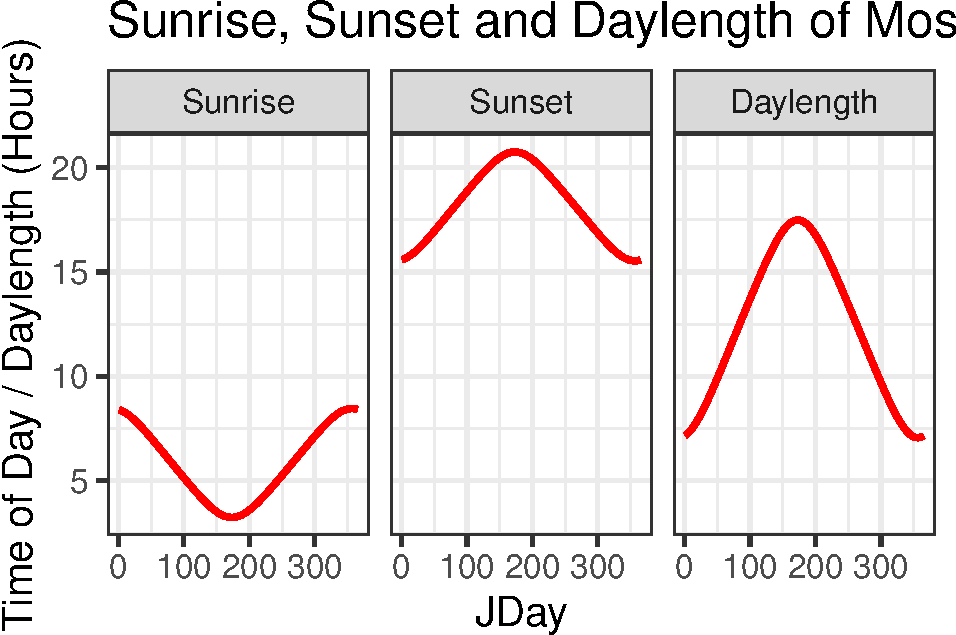
\includegraphics[width=0.8\linewidth]{Tree-Phenology_files/figure-latex/unnamed-chunk-16-1}

\hypertarget{task-2-3}{%
\section{Task 2}\label{task-2-3}}

\textbf{Produce an hourly dataset, based on idealized daily curves, for the KA\_weather dataset (included in chillR)}

\begin{quote}
The following two tasks were performed in a modified form. In order to demonstrate the application of the chillR package, it was decided to use a currently active weather station and use its data as a basis. Data on the weather station can be found in the table below.
\end{quote}

\begin{table}

\caption{\label{tab:unnamed-chunk-17}Weather Station Fuessenich}
\fontsize{10}{12}\selectfont
\begin{tabular}[t]{l|l|l|l}
\hline
Location & State & GPS & Gauß\_Krüger\\
\hline
Zuelpich - Fuessenich & North Rhine-Westphalia & 50.69527026369208, 6.615666577711913 & Rechtswert:2543500 Hochwert: 5617798\\
\hline
\end{tabular}
\end{table}

First, corresponding data must be read in. The data are already prepared.

\begin{Shaded}
\begin{Highlighting}[]
\NormalTok{Zuelpich_hourly =}\StringTok{ }\KeywordTok{read.table}\NormalTok{(}
  \StringTok{"weather_data/Weather_Zuelpich_2019_hourly.csv"}\NormalTok{,}
  \DataTypeTok{header =} \OtherTok{TRUE}\NormalTok{,}
  \DataTypeTok{sep =} \StringTok{","}
\NormalTok{)}

\NormalTok{Zuelpich_min_max =}\StringTok{ }\KeywordTok{read.table}\NormalTok{(}\StringTok{"weather_data/Weather_Zuelpich_2019.csv"}\NormalTok{,}
                              \DataTypeTok{header =} \OtherTok{TRUE}\NormalTok{,}
                              \DataTypeTok{sep =} \StringTok{","}\NormalTok{)}
\end{Highlighting}
\end{Shaded}

\begin{Shaded}
\begin{Highlighting}[]
\NormalTok{zuelpich_april =}\StringTok{ }\NormalTok{Zuelpich_hourly }\OperatorTok\StringTok{ }\KeywordTok{filter}\NormalTok{(}\StringTok{"2019-04-01 00:00:00"} \OperatorTok{<}\StringTok{ }\NormalTok{date) }\OperatorTok
\StringTok{  }\KeywordTok{filter}\NormalTok{(}\StringTok{"2019-04-05 00:00:00"} \OperatorTok{>}\StringTok{ }\NormalTok{date)}

\NormalTok{zuelpich_april}\OperatorTok{$}\NormalTok{date_new <-}\StringTok{ }\KeywordTok{as.POSIXct}\NormalTok{(zuelpich_april[, }\DecValTok{3}\NormalTok{])}
\NormalTok{zuelpich_april}\OperatorTok{$}\NormalTok{date_newnew =}\StringTok{ }\KeywordTok{as.Date}\NormalTok{(zuelpich_april[, }\DecValTok{3}\NormalTok{])}

\KeywordTok{kable}\NormalTok{(}\KeywordTok{head}\NormalTok{(zuelpich_april), }\DataTypeTok{caption =} \StringTok{"Dataset: zuelpich_april"}\NormalTok{) }\OperatorTok
\StringTok{  }\KeywordTok{kable_styling}\NormalTok{(}\StringTok{"striped"}\NormalTok{, }\DataTypeTok{position =} \StringTok{"left"}\NormalTok{, }\DataTypeTok{font_size =} \DecValTok{10}\NormalTok{)}
\end{Highlighting}
\end{Shaded}

\textbackslash begin\{table\}

\textbackslash caption\{\label{tab:unnamed-chunk-20}Dataset: zuelpich\_april\}
\fontsize{10}{12}\selectfont

\begin{tabular}[t]{r|r|l|l|l}
\hline
X & temperature & date & date\_new & date\_newnew\\
\hline
1412 & 3.4350000 & 2019-04-01 01:00:00 & 2019-04-01 01:00:00 & 2019-04-01\\
\hline
1413 & 2.0900000 & 2019-04-01 02:00:00 & 2019-04-01 02:00:00 & 2019-04-01\\
\hline
1414 & 1.2616667 & 2019-04-01 03:00:00 & 2019-04-01 03:00:00 & 2019-04-01\\
\hline
1415 & 0.6150000 & 2019-04-01 04:00:00 & 2019-04-01 04:00:00 & 2019-04-01\\
\hline
1416 & 0.0583333 & 2019-04-01 05:00:00 & 2019-04-01 05:00:00 & 2019-04-01\\
\hline
1417 & -0.3566667 & 2019-04-01 06:00:00 & 2019-04-01 06:00:00 & 2019-04-01\\
\hline
\end{tabular}

\textbackslash end\{table\}

\begin{quote}
Next, the lows and highs for the corresponding days must be determined from the data set containing hourly data.
\end{quote}

\begin{Shaded}
\begin{Highlighting}[]
\NormalTok{final <-}\StringTok{ }\NormalTok{zuelpich_april }\OperatorTok
\StringTok{  }\KeywordTok{group_by}\NormalTok{(}\DataTypeTok{Tag =} \KeywordTok{day}\NormalTok{(date_newnew)) }\OperatorTok
\StringTok{  }\KeywordTok{summarise}\NormalTok{(}
    \DataTypeTok{Mittel =}  \KeywordTok{round}\NormalTok{(}\KeywordTok{mean}\NormalTok{(temperature, }\DataTypeTok{na.rm =} \OtherTok{TRUE}\NormalTok{), }\DataTypeTok{digits =} \DecValTok{1}\NormalTok{),}
    \DataTypeTok{Tmax =} \KeywordTok{max}\NormalTok{(temperature),}
    \DataTypeTok{Tmin =} \KeywordTok{min}\NormalTok{(temperature)}
\NormalTok{  )}

\KeywordTok{kable}\NormalTok{(final, }\DataTypeTok{caption =} \StringTok{"Dataset:Tmean Tmax Tmin"}\NormalTok{)}\OperatorTok
\StringTok{  }\KeywordTok{kable_styling}\NormalTok{(}\StringTok{"striped"}\NormalTok{, }\DataTypeTok{position =} \StringTok{"left"}\NormalTok{, }\DataTypeTok{font_size =} \DecValTok{10}\NormalTok{)}
\end{Highlighting}
\end{Shaded}

\begin{table}

\caption{\label{tab:unnamed-chunk-21}Dataset:Tmean Tmax Tmin}
\fontsize{10}{12}\selectfont
\begin{tabular}[t]{r|r|r|r}
\hline
Tag & Mittel & Tmax & Tmin\\
\hline
1 & 7.7 & 17.810000 & -0.420000\\
\hline
2 & 9.5 & 17.096667 & 2.693333\\
\hline
3 & 7.6 & 9.983333 & 5.481667\\
\hline
4 & 5.7 & 7.763333 & 3.566667\\
\hline
\end{tabular}
\end{table}

\begin{quote}
Next, the dataset containing hourly temperature values must be extended with a column that will later represent the daily high and low values. First, the new column \texttt{Tmax\_Tmin} is filled with ``NAs''. Then the maximum and minimum values are taken from the previously generated dataset \texttt{final}. These values are compared with the hourly values. If they match, the maximum or minimum value found is written to the previously created column \texttt{Tmax\_Tmin}. In this way, the daily maximum and minimum values are placed in the table \texttt{zuelpich\_april} at the same place where they were also measured.
\end{quote}

  \bibliography{book.bib,packages.bib}

\end{document}
